\section{Cascaded Shadow Maps}

\begin{figure}[h]
    \centering
    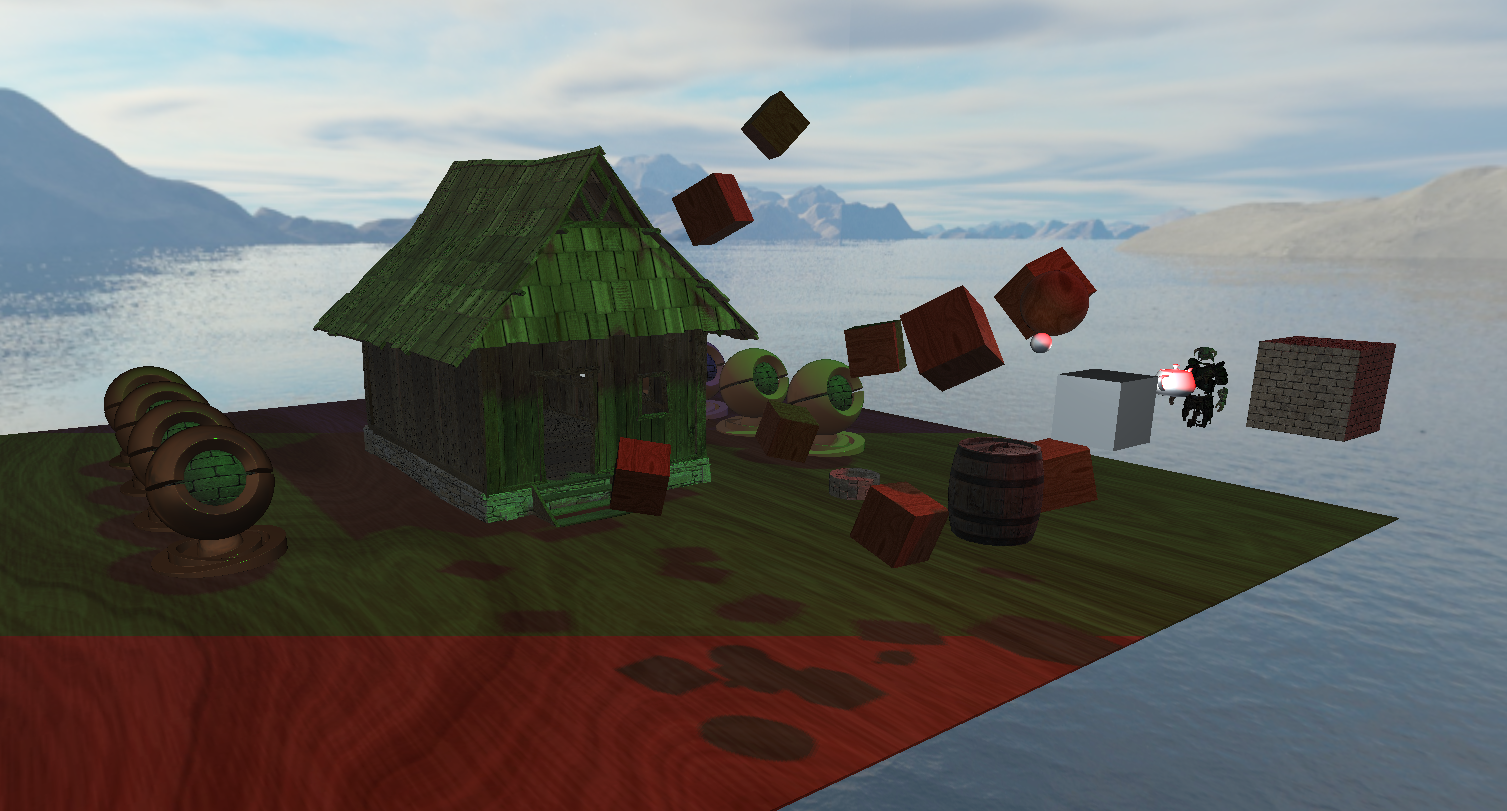
\includegraphics[scale=0.25, clip=true]{./image/csmsplits.png}
    \caption{Visualized frustum splits}
\label{fig:csmsplits}
\end{figure}

\begin{figure}[b]
    \centering
    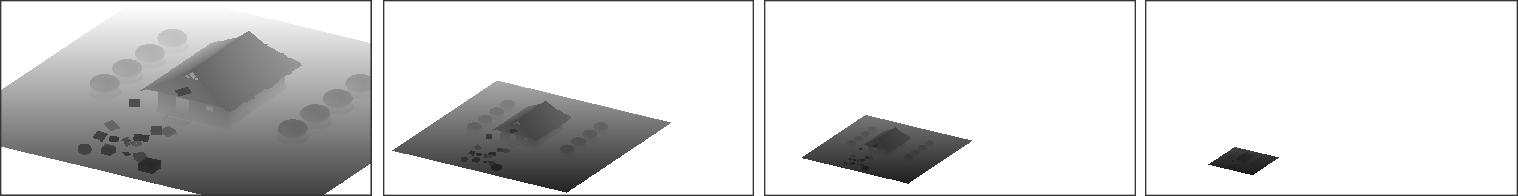
\includegraphics[scale=0.3, clip=true]{./image/csmbufs.png}
    \caption{Depth maps for each frustum split}
\label{fig:csmbufs}
\end{figure}

In order to implement shadows in the scenes the use of some Shadow Mapping technique was required.
The simple shadow mapping algorithm would not be sufficient for large space scenes. Using just
a single shadowmap leads to difficulties in adjusting the shadow map to avoid surface acne and aliasing
problems. Also this would require a very high and impractical resolution in order capture both large
space scenes and being able to show desirable detail. Cascaded Shadow Maps is an approach that helps bypass
these problems by providing higher resolution of the depth texture near the viewer an lower resolution far
away. This is achieved by splitting the camera view frustum and creating a separate depth-map for each
partition (see Figures~\ref{fig:csmsplits},\ref{fig:csmbufs}). The algorithm is composed of two main parts:

\begin{enumerate}
\item For every frustum split render the scene depth from the light pov
\item While rendering the scene from the camera pov, pick and use the matching shadow map for the current
    fragment's Z value
\end{enumerate}

For the creation of each depth map, firstly the split planes, view and projection matrices for each split
must be calculated. For each split the procedure goes like this:

\begin{enumerate}
\item Calculate near and far splits
\item Create the projection for the split using previously calculated near and far values
\item Extract the split frustum points by multiplying the inverse projection-view matrix
    with each of the vertices of an NDC cube (note that the prespective division must
    be performed manually)
\item Find the centroid of the previously calculated split frustum
\item Create the view matrix with the eye being the light position looking towards the centroid
\item Transform the split vertices to the light view space
\item Find the frustum bounding box in view space
\item Create an orthogonal projection matrix with the corners of the previously calculated bounding box
\item Save calculated split projection, view matrices and near, far planes for later use
\end{enumerate}

Next we need to render the scene for each split in order to create the shadow maps.
In each split render we transform the vertices by its respective projection and view matrices
that we have previously calculated. Note that the final stored depths must be in linear space.
A intermediate geometry shader with invocations number set to the split number can be also used
to avoid multiple draws. Before rendering the shadow maps it is also adviced to switch to front
face culling to avoid peter-panning effects.

When using the shadow maps in the shading phase, all it needs to be done is choose the shadow
map layer to be used according to the depth of the current vertex in view space. After that
the fragment must be transformed from world to light space and check if it is in shadow like
the normal shadowmapping algorithm. Optional PCF can be applied after that.
